\documentclass[10pt,english]{beamer}
%\documentclass[english,handout]{beamer} % For handouts
\input{../metropolis_preamble.tex}
\input{../macros.tex}
%\usepackage{extendedalt}
%\usepackage{animate} % Animations
%\usepackage{../lindsten}
%\usepackage{movie15}

\hypersetup{
  colorlinks=true, urlcolor=blue, linkcolor=red
}
%[colorlinks=true, urlcolor=blue, linkcolor=red]{hyperref}


\title{732G57  Maskininlärning för statistiker }
\subtitle{Föreläsning 2}
\date{}
\author{Josef Wilzén \\ IDA, Linköping University, Sweden}
\titlegraphic{\hfill
\includegraphics[height=1.2cm]{../LiU_primary_black.pdf}}
%\institute{Joint work with\dots}


%% MY DEF %%
\newcommand{\itm}[1]{\mathrm{Item}_{#1}}
\newcommand{\pausa}{\pause}
%\renewcommand{\pausa}{}


\newenvironment{nscenter}
 {\parskip=0pt\par\nopagebreak\centering}
 {\par\noindent\ignorespacesafterend}

\begin{document}

\maketitle

\begin{frame}{Dagens föreläsning}
    
    \begin{itemize}
        \item Modellval
        \item Logistisk regression
        \item Klassificering: utvärdering
        \item Modellval för linjär regression
    \end{itemize}

\end{frame}

\begin{frame}{Modellval}
    
    \begin{itemize}
        \item Vi söker en modell som \textbf{generaliserar} väl.
        \begin{itemize}
            \item Med generalisering menas att den ska fungera bra på ny data.
        \end{itemize}
        \item En flexibel (komplex) modell har lättare att överanpassa.
        \item Vad är ''komplexitet''?
        \begin{itemize}
            \item Linjär modell: Antal variabler, interaktioner, transformationer etc
            \item Splines: frihetsgrader
            \item Neurala nätverk: Bredd och djup av modellen
            \item Trädmodeller: Djupet/antal löv
        \end{itemize}
    \end{itemize}

\end{frame}

\begin{frame}{Regularisering}

    Regularisering är ett sätt att motverka överanpassning.

    \begin{itemize}
        \item Idé att hindra modellen att bli för komplex.
        \item Regularisering $\approx$ "begränsning"
        \item Ger förhoppningsvis bättre generaliseringsfel.
        \item \textbf{Mycket viktigt tema inom maskininlärning}
        \item Görs på olika sätt för olika modeller.
    \end{itemize}

    Idén är att
    \begin{equation*}
        \text{Flexibel modell} + \text{regularisering} = \text{en bra modell}
    \end{equation*}

    Kommer prata mer om detta senare.

\end{frame}

\begin{frame}{Regression och Klassificering}
    
    Två klassiska problem är regression och klassificering.

    \begin{itemize}
        \item Regression: Prediktera en variabel $y$, oftast $y$ kontinuerlig. Bruset $\varepsilon$ är:
        \begin{itemize}
            \item Vanligast är normalfördelat.
            \item Alternativt, t-fördelning, Gamma, Log-normal,\dots
            \item Kan också vara disktet, Poisson, Negativ binomial,\dots
        \end{itemize}
        \item Fördelningen ger felfunktionen.
        \item Klassificering: $y$ är kategorisk med 2 eller flera utfall:
        \begin{itemize}
            \item Binär: logistisk/probit regression
            \item Fler klasser: Multinomial logistisk/probit regression
            \item Kommer diskutera fler metoder senare
            \item Hur skapar vi en felfunktion? Utvärdering?
        \end{itemize}
    \end{itemize}

\end{frame}


\begin{frame}{Logistisk regression}

\begin{itemize}
    \item Responsvariabeln antas vara Bernoullifördelad:
    \[
        y_i \sim \operatorname{Bernoulli}(p_i),
        \qquad
        \mathbb{P}(y_i=1)=p_i.
    \]

    \item Logitlänken kopplar sannolikheten till den linjära prediktorn:
    \[
        \log\left(\frac{p_i}{1-p_i}\right)
        =
        \boldsymbol{x}_i^\top\boldsymbol{\beta}.
    \]

    \item Detta ger
    \[
        p_i
        =
        \frac{\exp(\boldsymbol{x}_i^\top\boldsymbol{\beta})}
        {1+\exp(\boldsymbol{x}_i^\top\boldsymbol{\beta})}.
    \]

    \item Likelihoodfunktionen för oberoende observationer är
    \[
        L(\boldsymbol{\beta})
        =
        \prod_{i=1}^{n}
        p_i^{y_i}(1-p_i)^{1-y_i}.
    \]

    \item Parametrarna skattas genom att maximera likelihoodfunktionen:
    \[
        \widehat{\boldsymbol{\beta}}
        =
        \arg\max_{\boldsymbol{\beta}} L(\boldsymbol{\beta}).
    \]
\end{itemize}

\end{frame}



\begin{frame}{Skattning i logistisk regression}

Parametrarna skattas genom att maximera log-likelihoodfunktionen:

\[
\widehat{\boldsymbol{\beta}}
=
\arg\max_{\boldsymbol{\beta}}
\ell(\boldsymbol{\beta}),
\]

där

\[
\ell(\boldsymbol{\beta})
=
\sum_{i=1}^{n}
\left[
y_i\log(p_i)
+
(1-y_i)\log(1-p_i)
\right],
\]

och

\[
p_i
=
\frac{\exp(\boldsymbol{x}_i^\top\boldsymbol{\beta})}
{1+\exp(\boldsymbol{x}_i^\top\boldsymbol{\beta})}.
\]




\end{frame}


\begin{frame}{Skattning i logistisk regression}

Optimeringsalgoritmer formuleras ofta för minimering. Därför kan vi
minimera den negativa log-likelihoodfunktionen:

\[
-\ell(\boldsymbol{\beta})
=
-\sum_{i=1}^{n}
\left[
y_i\log(p_i)
+
(1-y_i)\log(1-p_i)
\right].
\]


\end{frame}


\begin{frame}{Skattning i logistisk regression}

Vanliga optimeringsmetoder:

\begin{itemize}
    \item Gradient descent och varianter av gradient descent
    \item Newton--Raphsons metod $\rightarrow$ använder hessianen
    \item Fisher scoring $\rightarrow$ använder förväntade hessianen
    \item Iteratively Reweighted Least Squares (IRLS)
\end{itemize}

\begin{block}{Logistisk regression i R}
\texttt{glm(..., family = binomial)} använder iterativt viktade
minsta kvadratmetoden (IRLS), vilket för logistisk regression
motsvarar Fisher scoring.
\end{block}

\end{frame}



\begin{frame}{Multinomial logistisk regression: data}

    Antag att responsvariabeln har tre klasser:

    \[
        Y_i \in \{1,2,3\},
        \qquad
        K=3,
    \]

    och att vi har fyra förklarande variabler:

    \[
        x_1,\;x_2,\;x_3,\;x_4.
    \]

    \medskip

    För tre observationer kan designmatrisen, inklusive intercept, vara

    \[
        X
        =
        \begin{pmatrix}
            1 & 1 & 0 & 2 & -1 \\
            1 & 0 & 1 & 1 &  0 \\
            1 & 1 & 1 & 0 &  2
        \end{pmatrix}.
    \]

    \begin{itemize}
        \item Första kolumnen motsvarar interceptet.
        \item Övriga kolumner motsvarar \(x_1,x_2,x_3,x_4\).
        \item Varje rad motsvarar en observation.
    \end{itemize}

\end{frame}



\begin{frame}{One-hot-kodning av responsvariabeln}

    Antag att de tre observationerna tillhör klasserna

    \[
        \boldsymbol{y}
        =
        \begin{pmatrix}
            1 \\
            2 \\
            3
        \end{pmatrix}
        \qquad
        \Longrightarrow
        \qquad
        Y
        =
        \begin{pmatrix}
            1 & 0 & 0 \\
            0 & 1 & 0 \\
            0 & 0 & 1
        \end{pmatrix}.
    \]

    Kolumnerna i \(Y\) motsvarar klasserna \(k=1,2,3\).

    \medskip

    Elementen i den one-hot-kodade responsmatrisen definieras som

    \[
        y_{ik}
        =
        \begin{cases}
            1, & \text{om observation \(i\) tillhör klass \(k\),} \\
            0, & \text{annars.}
        \end{cases}
    \]

    \begin{itemize}
        \item Varje rad motsvarar en observation.
        \item Varje kolumn motsvarar en klass.
        \item Varje rad summerar till ett.
    \end{itemize}

\end{frame}





\begin{frame}{Referensklass-formulering}

    En vanlig formulering väljer en av de \(K\) klasserna som
    referensklass.

    \medskip

    Om klass \(k=3\) är referensklass modelleras

    \[
        \log
        \left(
            \frac{P(Y_i=1\mid\boldsymbol{x}_i)}
                 {P(Y_i=3\mid\boldsymbol{x}_i)}
        \right)
        =
        \beta_{01}
        +
        \boldsymbol{x}_i^{\mathsf T}\boldsymbol{\beta}_1,
    \]

    och

    \[
        \log
        \left(
            \frac{P(Y_i=2\mid\boldsymbol{x}_i)}
                 {P(Y_i=3\mid\boldsymbol{x}_i)}
        \right)
        =
        \beta_{02}
        +
        \boldsymbol{x}_i^{\mathsf T}\boldsymbol{\beta}_2.
    \]

    \begin{itemize}
        \item Endast \(K-1\) linjära prediktorer behöver skattas.
        \item Koefficienterna tolkas relativt referensklassen.
        \item Ett byte av referensklass ändrar koefficienterna, men inte
              modellens skattade klassannolikheter.
    \end{itemize}

\end{frame}


\begin{frame}{Softmax-formulering}

    En linjär prediktor används för varje klass:

    \[
        \eta_{ik}
        =
        \beta_{0k}
        +
        \boldsymbol{x}_i^{\mathsf T}\boldsymbol{\beta}_k,
        \qquad
        k=1,\ldots,K.
    \]

    Klassannolikheterna beräknas med softmax-funktionen:

    \[
        p_{ik}
        =
        P(Y_i=k\mid\boldsymbol{x}_i)
        =
        \frac{\exp(\eta_{ik})}
             {\displaystyle
              \sum_{j=1}^{K}\exp(\eta_{ij})}.
    \]

    Softmax ger giltiga klassannolikheter:

    \[
        0<p_{ik}<1,
        \qquad
        \sum_{k=1}^{K}p_{ik}=1.
    \]
  \medskip
  I \texttt{glmnet} använd \texttt{family = "multinomial"} En koefficientvektor
        skattas för varje klass.


\end{frame}

\begin{frame}{Exempel på skattade koefficienter}

    Antag att följande koefficientmatris har skattats:

    \[
        \widehat{\boldsymbol{\Theta}}
        =
        \begin{array}{c|rrr}
                            & k=1  & k=2  & k=3  \\ \hline
            \text{Intercept} & 0.4  & -0.2 & -0.2 \\
            x_1              & 0.6  & -0.3 & -0.3 \\
            x_2              & -0.3 & 0.5  & -0.2 \\
            x_3              & 0.2  & -0.4 & 0.2  \\
            x_4              & -0.1 & 0.1  & 0
        \end{array}.
    \]

    Varje kolumn innehåller koefficienterna för en klass:

    \[
        \widetilde{\boldsymbol{\beta}}_k
        =
        \begin{pmatrix}
            \beta_{0k} \\
            \beta_{1k} \\
            \vdots \\
            \beta_{4k}
        \end{pmatrix},
        \qquad
        k=1,2,3.
    \]


\end{frame}


\begin{frame}{Exempel på skattade koefficienter}

    

    De linjära prediktorerna för observation \(i\) blir

    \[
        \widehat{\boldsymbol{\eta}}_i
        =
        \widehat{\boldsymbol{\Theta}}^{\mathsf T}
        \widetilde{\boldsymbol{x}}_i,
        \qquad
        \widetilde{\boldsymbol{x}}_i
        =
        \begin{pmatrix}
            1 & x_{i1} & x_{i2} & x_{i3} & x_{i4}
        \end{pmatrix}^{\mathsf T}.
    \]

\end{frame}


\begin{frame}{Beräkning av klassannolikheter}

    Betrakta en observation med

    \[
        \widetilde{\boldsymbol{x}}_i
        =
        \begin{pmatrix}
            1 & 1 & 0 & 1 & 0
        \end{pmatrix}^{\mathsf T}.
    \]

    De linjära prediktorerna beräknas som

    \[
        \widehat{\boldsymbol{\eta}}_i
        =
        \widehat{\boldsymbol{\Theta}}^{\mathsf T}
        \widetilde{\boldsymbol{x}}_i
        =
        \begin{pmatrix}
            1.2 \\
            -0.9 \\
            -0.3
        \end{pmatrix}.
    \]

    Softmax-funktionen ger

    \[
        \widehat{p}_{ik}
        =
        \frac{\exp(\widehat{\eta}_{ik})}
             {\displaystyle
              \sum_{j=1}^{3}\exp(\widehat{\eta}_{ij})}.
    \]

    
\end{frame}


\begin{frame}{Beräkning av klassannolikheter}

    

    För observation \(i\) får vi därför

    \[
        \begin{pmatrix}
            \widehat{p}_{i1} \\
            \widehat{p}_{i2} \\
            \widehat{p}_{i3}
        \end{pmatrix}
        =
        \frac{1}
             {e^{1.2}+e^{-0.9}+e^{-0.3}}
        \begin{pmatrix}
            e^{1.2} \\
            e^{-0.9} \\
            e^{-0.3}
        \end{pmatrix}
        \approx
        \begin{pmatrix}
            0.743 \\
            0.091 \\
            0.166
        \end{pmatrix}.
    \]

    Modellen predikterar klass \(1\), eftersom

    \[
        \widehat{p}_{i1}
        =
        \max_{k\in\{1,2,3\}}\widehat{p}_{ik}.
    \]

\end{frame}


\begin{frame}{Hur påverkar koefficienterna prediktionen?}

    Varje klass \(k\) har en egen linjär prediktor:

    \[
        \eta_{ik}
        =
        \beta_{0k}
        +
        \sum_{j=1}^{p} x_{ij}\beta_{jk}.
    \]

    \begin{itemize}
        \item En positiv \(\beta_{jk}\) innebär att ett större värde på
              \(x_j\) ökar den linjära prediktorn för klass \(k\).

        \item En negativ \(\beta_{jk}\) innebär att ett större värde på
              \(x_j\) minskar den linjära prediktorn för klass \(k\).

        \item Softmax jämför de linjära prediktorerna för alla klasser:
              \[
                  p_{ik}
                  =
                  \frac{\exp(\eta_{ik})}
                       {\displaystyle
                        \sum_{r=1}^{K}\exp(\eta_{ir})}.
              \]

        \item En klass med högre \(\eta_{ik}\) får en högre skattad
              sannolikhet relativt övriga klasser.
    \end{itemize}

    

\end{frame}


\begin{frame}{Hur påverkar koefficienterna prediktionen?}



    \begin{block}{Predikterad klass}
        Observation \(i\) klassificeras till den klass som har högst
        skattad sannolikhet:
        \[
            \widehat{y}_i
            =
            \arg\max_{k\in\{1,\ldots,K\}}
            \widehat{p}_{ik}.
        \]
    \end{block}

\end{frame}

\begin{frame}{Log-likelihood}

    För observation \(i\) och klass \(k\) är

    \[
        y_{ik}
        =
        \begin{cases}
            1, & \text{om observation \(i\) tillhör klass \(k\),} \\
            0, & \text{annars.}
        \end{cases}
    \]

    Likelihoodfunktionen är

    \[
        L(\boldsymbol{\Theta})
        =
        \prod_{i=1}^{n}
        \prod_{k=1}^{K}
        p_{ik}^{\,y_{ik}}.
    \]

    Log-likelihoodfunktionen blir

    \[
        \ell(\boldsymbol{\Theta})
        =
        \sum_{i=1}^{n}
        \sum_{k=1}^{K}
        y_{ik}\log(p_{ik}).
    \]

\end{frame}


\begin{frame}{Log-likelihood}



    Parametrarna skattas genom att maximera log-likelihooden:

    \[
        \widehat{\boldsymbol{\Theta}}
        =
        \arg\max_{\boldsymbol{\Theta}}
        \ell(\boldsymbol{\Theta}).
    \]

    \begin{block}{One-hot-kodning}
        Varje observation bidrar endast med logaritmen av den
        skattade sannolikheten för observationens faktiska klass.
    \end{block}

\end{frame}


\begin{frame}{Förväxlingsmatris}
\begin{center}
    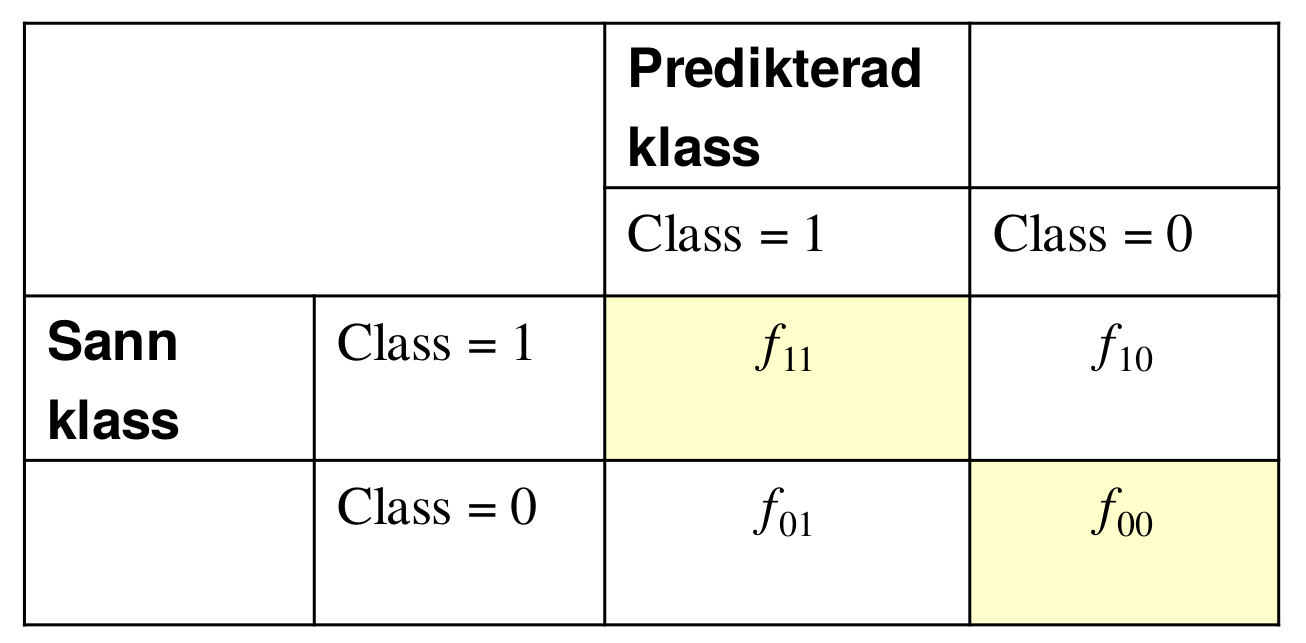
\includegraphics[width=0.7\textwidth]{figs/Screenshot at 2020-08-18 12-24-31.png}
\end{center}

\begin{itemize}
    \item Träffsäkerhet:
    \begin{equation*}
        \operatorname{T} = \frac{f_{11} + f_{00}}{f_{11} + f_{10} + f_{01} + f_{00}}.
    \end{equation*}
    \item Felkvot (error rate):
    \begin{equation*}
        \operatorname{E} = \frac{f_{10} + f_{01}}{f_{11} + f_{10} + f_{01} + f_{00}}.
    \end{equation*}
    \item Obalanserade klasser? Olika typer av fel är olika allvarliga?
\end{itemize}
    
\end{frame}

\begin{frame}{Förväxlingsmatris}
    \begin{center}
        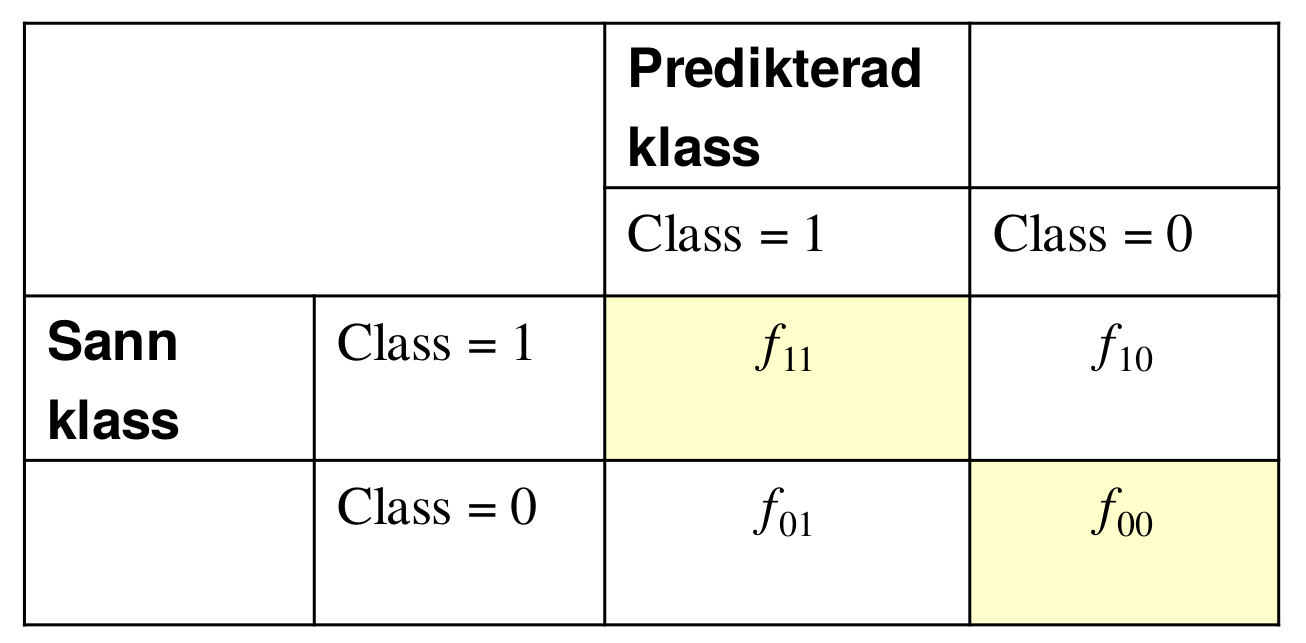
\includegraphics[width=0.7\textwidth]{figs/Screenshot at 2020-08-18 12-24-31.png}
    \end{center}
    
    \begin{itemize}
        \item Sensitivitet (recall, hit rate, true positive rate):
        \begin{equation*}
            \operatorname{TPR} = \frac{f_{11} }{f_{11} + f_{10}}.
        \end{equation*}
        \item Specificitet (selectivity, true negative rate):
        \begin{equation*}
            \operatorname{TNR} = \frac{f_{00}}{f_{00} + f_{01}}.
        \end{equation*}
        \item Beräknas klassvis.
    \end{itemize}
        
\end{frame}

\begin{frame}{F-score}
    
    \begin{itemize}
        \item  Precision (positive predictive value):
        \begin{equation*}
            \operatorname{PPV} = \frac{f_{11}}{f_{11} + f_{01}}.
        \end{equation*}
        \item F-score är ett mått av träffsäkerhet baserat på precision och sensitivitet.
        \begin{equation*}
            F_{\beta} = (1 + \beta^2) \frac{\operatorname{PPV} \cdot \operatorname{TPR}}{\beta^2 \cdot \operatorname{PPV} + \operatorname{TPR}}
        \end{equation*}
        \item Vanligt med $\beta=1$ vilket ger (harmoniska medelvärdet)
        \begin{equation*}
            F_1 = 2 \frac{\operatorname{PPV} \cdot \operatorname{TPR}}{\operatorname{PPV} + \operatorname{TPR}}
        \end{equation*}
        \item F-score är mellan 0 och 1, högre är bättre.
        \item $\beta$ säger hur du värderar precision och sensivitet.
        \item Beräknas klassvis.
    \end{itemize}

\end{frame}


\begin{frame}{Klassificering - utvärdering}


\begin{itemize}
    \item Vanligt att skatta modellen med en felfunktion (tex negativa loglikelihoodfunktionen/cross entropy loss) och sen utvärdera med andra mått (felkvot, sensitivitet, specificitet etc)
    \item Problemet och strukturen på data avgör vilka mått som är lämpliga
    \item Förväxlingsmatris - fler klasser, se separat dokument: \href{https://raw.githubusercontent.com/STIMALiU/732G57_DM/master/other/confusion\%20matrix\%20classification\%20evaluation\%20metrics.pdf}{kommer snart}
\end{itemize}
    
\end{frame}



% \begin{frame}{Generaliserade linjära modeller}
% 
%     Antag att data $\mathbf{y} = y_1, y_2, \ldots, y_n$ är oberoende observationer från sannolikhetsfördelning från \href{https://en.wikipedia.org/wiki/Exponential_family}{exponentialfamiljen}.
% 
%     Vi har en linjär prediktor $\mathbf{X} \beta$ samt en länkfunktion $g$ som kopplar ihop prediktorn med medelvärdet $\mu$ genom
%     \begin{equation*}
%         g(\mu) = \mathbf{X} \beta.
%     \end{equation*}
%     
%     Tar "vanlig" linjär regression till andra typer av responsvariabler
%     \begin{itemize}
%         \item Kontinuerlig: Normal, t, gamma, log-normal
%         \item Binär: Logistisk regression
%         \item Nominell: Multinomiell logistisk regression
%         \item Frekvensdata: Poissonregression, Negativ binomialregression
%     \end{itemize}
% \end{frame}
% 
% \begin{frame}{Generaliserade linjära modeller - Exempel}
% 
%     \myheading{Linjär regression}
%     \begin{itemize}
%         \item Likelihood: Normal
%         \item L\"ankfunktion: identitetsfunktionen
%         \item SKattas genom att minimera:
%         \begin{equation*}
%             \operatorname{RSS} = \sum_{i=1}^{n} \left( y_i - \beta_0 - \sum_{j=1}^{p} \beta_j x_{ij} \right)^2
%         \end{equation*}
%     \end{itemize}
% 
% \end{frame}
% 
% \begin{frame}{Generaliserade linjära modeller - Exempel}
%     \myheading{Logistisk regression}
%     \begin{itemize}
%         \item Likelihood: Bernoulli ($y$ kan vara 0 eller 1, $\mathbb{P}(y = 1) = p$)
%         \item L\"ankfunktion: Logit,
%         \begin{equation*}
%             g(\mu) = \log\left( \frac{\mu}{1-\mu} \right)
%         \end{equation*}
%         \item Skattas med att maximera likelihoodfunktionen (MLE)
%     \end{itemize}
% \end{frame}

% \begin{frame}{Generaliserade linjära modeller - Exempel}
%     \myheading{Multinominell logistisk regression}
%     \begin{itemize}
%         \item Likelihood: Kategorisk ($y$ kan ta $K$ olika värden, $\mathbb{P}(y = k) = p_k$)
%         \item L\"ankfunktion: Logit,
%         \begin{equation*}
%             g(\mu) = \log\left( \frac{\mu}{1-\mu} \right)
%         \end{equation*}
%         \item Skattas med att maximera MLE
%     \end{itemize}
% \end{frame}

\begin{frame}{Modellval för linjära regression}

    Utgå ifrån: $y$ kontinuerlig med normal likelihood.

    Vi har ett antal förklarande variabler $\mathbf{x} = (x_1, \ldots, x_p)$. Vill hitta parametrar/modell som ger minst generaliseringsfel.

    Två alternativ:
    \begin{itemize}
        \item Alternativ 1: Välj ut en delmängd av variablerna.
        \begin{itemize}
            \item Best subset, forward selection, backward selection
        \end{itemize}
        \item Alternativ 2: Behåll alla variabler men begränsa parametrarna.
        \begin{itemize}
            \item Regularisering, Ridge och Lasso.
        \end{itemize}  
    \end{itemize}
    
\end{frame}

\begin{frame}{Utvärderingsmått}
    Om vi har flera modeller, hur jämför vi dessa?

    Två alternativ:
    \begin{itemize}
        \item Indirekt skatta testfelet
        \begin{itemize}
            \item Utgå från träningsmängden
            \item Försök att minska den bias som uppstår när vi inte använder all data.
        \end{itemize}
        \item Direkt skatta testfelet
        \begin{itemize}
            \item Valideringsdata
            \item Korsvalidering
        \end{itemize}
    \end{itemize}
\end{frame}

\begin{frame}{Indirekt skatta testfelet}
    MSE på träningsdatan underskattar "riktiga" MSE värdet, kan inte användas för att välja modell.

    Idé: justera träningsfelet för att ta hänsyn till detta. 

    \begin{equation*}
        C_p = \frac{1}{n} (\operatorname{RSS} + 2 d \hat{\sigma}^2),
    \end{equation*}

    Litet $C_p$ är bäst.

    \begin{equation*}
        \text{adjusted R}^2 = 1 - \frac{\operatorname{RSS}/(n-d-1)}{\operatorname{TSS}/(n-1)},
    \end{equation*}
    där
    \begin{equation*}
        \operatorname{TSS} = \sum_{i=1}^{n}(y_i - \bar{y})^2.
    \end{equation*}

    Stort $\text{adjusted R}^2$ är bäst.
\end{frame}

\begin{frame}{Indirekt skatta testfelet}
    
    Tre andra mått AIC, BIC och HQIC är baserade på MLE skattning ev modeller.

    Låt $\log(\hat{L})$ vara log-likelihood för optimala parametervärden.

    \begin{align*}
        \operatorname{AIC} &= 2 d - 2 \log(\hat{L}) \\
        \operatorname{BIC} &= d \cdot \log(n) - 2 \log(\hat{L}) \\
        \operatorname{HQIC} &= d \cdot \log(\log(n)) - 2 \log(\hat{L}) 
    \end{align*}

    Lågt värde är bättre.

\end{frame}

\begin{frame}{Indirekt skatta testfelet}
    
    \myheading{Linjär Regression}

    \begin{align*}
        \operatorname{AIC} &= \frac{1}{n \hat{\sigma}^2} (\operatorname{RSS} + 2 d \hat{\sigma}^2) \\
        \operatorname{BIC} &= \frac{1}{n \hat{\sigma}^2} (\operatorname{RSS} + \log(n) d \hat{\sigma}^2) \\
        \operatorname{HQIC} &= \frac{1}{n \hat{\sigma}^2} (\operatorname{RSS} + \log(\log(n)) d \hat{\sigma}^2)
    \end{align*}

    För linjär regression är $C_p \propto \operatorname{AIC}$.

\end{frame}

% \begin{frame}{Best subset selection}
%     \begin{nscenter}
%         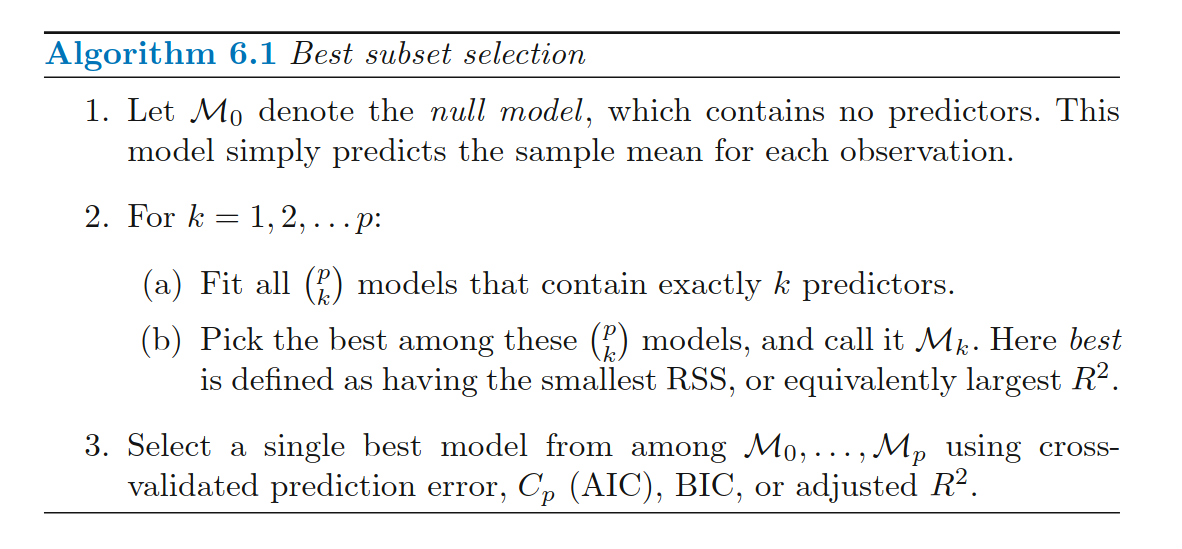
\includegraphics[width=\textwidth]{figs/best subset selection.png}
%     \end{nscenter}
%     Bild från kursboken "An Introduction to Statistical Learning with Applications in R".
% 
% \end{frame}

\begin{frame}{Forward selection}
    \begin{nscenter}
        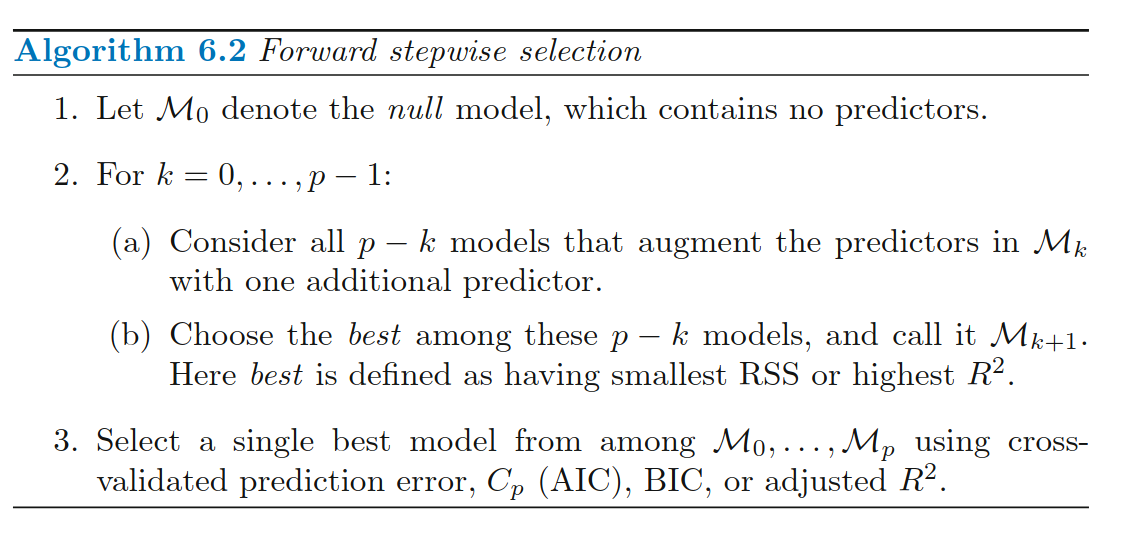
\includegraphics[width=\textwidth]{figs/Forward stepwise selection.png}
    \end{nscenter}
    Bild från kursboken "An Introduction to Statistical Learning with Applications in R".

\end{frame}

% \begin{frame}{Backward selection}
%     \begin{nscenter}
%         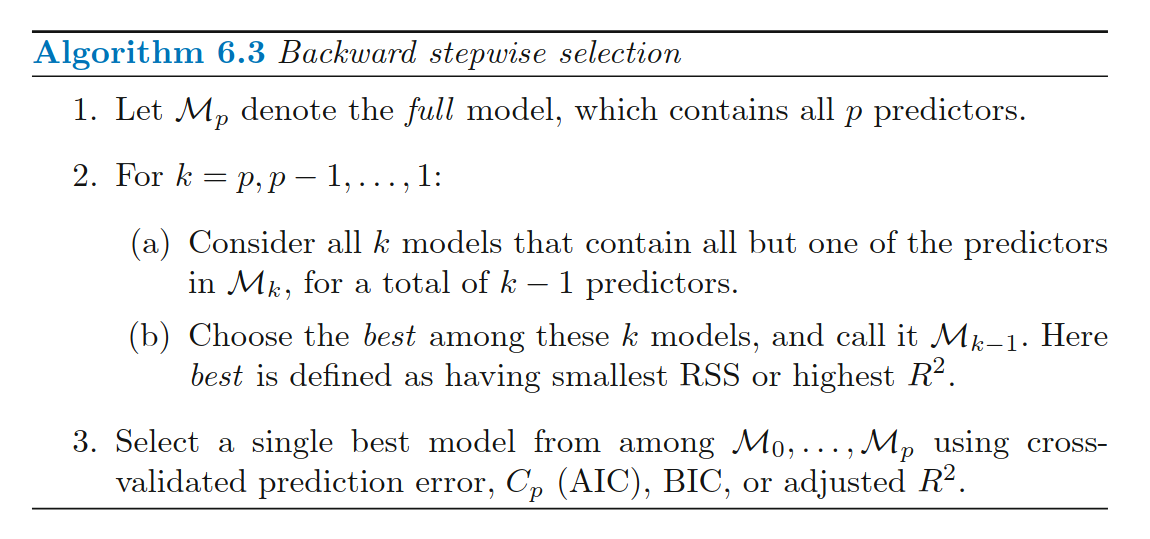
\includegraphics[width=\textwidth]{figs/Backward stepwise selection.png}
%     \end{nscenter}
%     Bild från kursboken "An Introduction to Statistical Learning with Applications in R".
% 
% \end{frame}

\begin{frame}{Krympning (Shrinkage)}
    
    Idé: begränsa hur stora parametrarna får vara.
    \begin{itemize}
        \item Straffa stora parametrar
        \item Ändra deras värdemängd
    \end{itemize}
    Vanligaste metoderna:
    \begin{itemize}
        \item Ridge: $l^2$-norm
        \item Lasso: $l^1$-norm
    \end{itemize}

    Kom ihåg att standardisera era förklarande variabler först innan krympning!

\end{frame}

\begin{frame}{Ridge Regression}

    I vanliga regression minimerar vi
    \begin{equation*}
        f(\beta) = \operatorname{RSS} = \sum_{i=1}^{n}\left(y_i - \beta_0 - \sum_{j=1}^{p}\beta_j x_{ij}\right)^2
    \end{equation*}
    I Ridge lägger vi till $l^2$-norm på $\beta$ vilket ger
    \begin{equation*}
        f_{\text{Ride}}(\beta) = \sum_{i=1}^{n}\left(y_i - \beta_0 - \sum_{j=1}^{p}\beta_j x_{ij}\right)^2 + \lambda \sum_{j=1}^{p} \beta_j^2, \quad \lambda \geq 0.
    \end{equation*}
    $\lambda$ är en \textbf{hyperparameter} som vi behöver sätta.

    Notera att $\beta_0$ inte påverkas.
    
\end{frame}

\begin{frame}{Ridge Regression}

    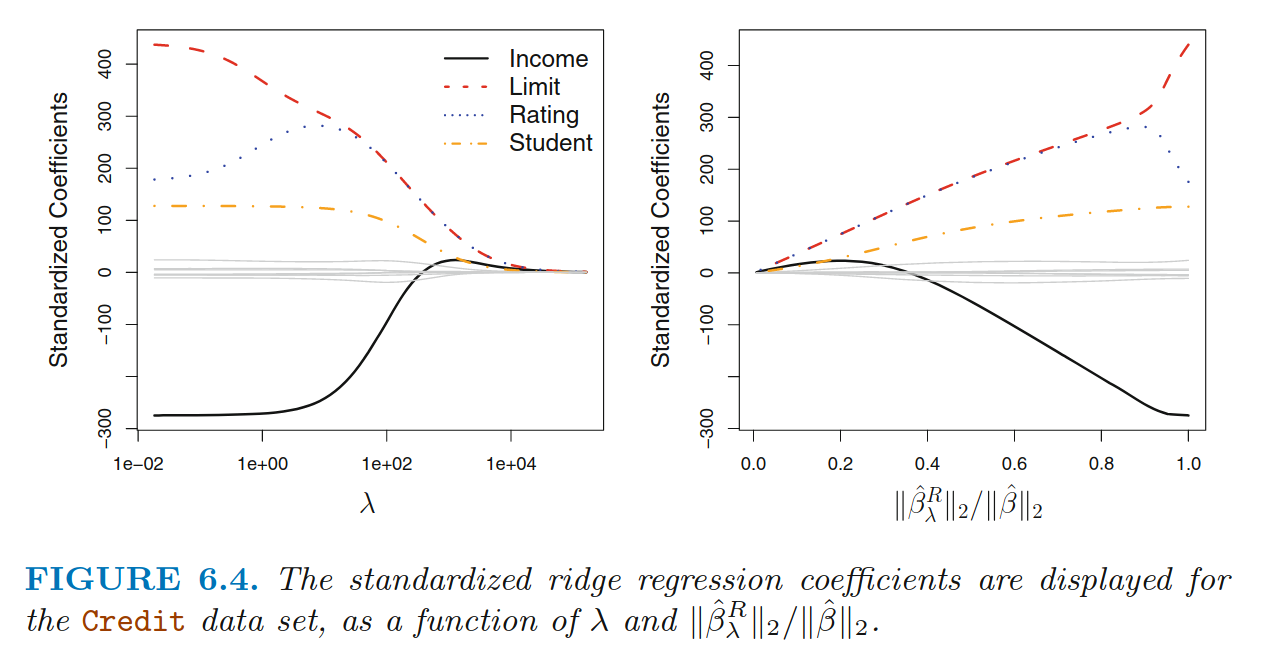
\includegraphics[width=\textwidth]{figs/standardized ridge regression coefficients.png}
    
\end{frame}

\begin{frame}{Lasso Regression}
    I vanliga regression minimerar vi
    \begin{equation*}
        f(\beta) = \operatorname{RSS} = \sum_{i=1}^{n}\left(y_i - \beta_0 - \sum_{j=1}^{p}\beta_j x_{ij}\right)^2
    \end{equation*}
    I Ridge lägger vi till $l^1$-norm på $\beta$ vilket ger
    \begin{equation*}
        f_{\text{Ride}}(\beta) = \sum_{i=1}^{n}\left(y_i - \beta_0 - \sum_{j=1}^{p}\beta_j x_{ij}\right)^2 + \lambda \sum_{j=1}^{p} |\beta_j|, \quad \lambda \geq 0.
    \end{equation*}
    $\lambda$ är en \textbf{hyperparameter} som vi behöver sätta.

    Notera att $\beta_0$ inte påverkas.
\end{frame}

\begin{frame}{Lasso Regression}
    
    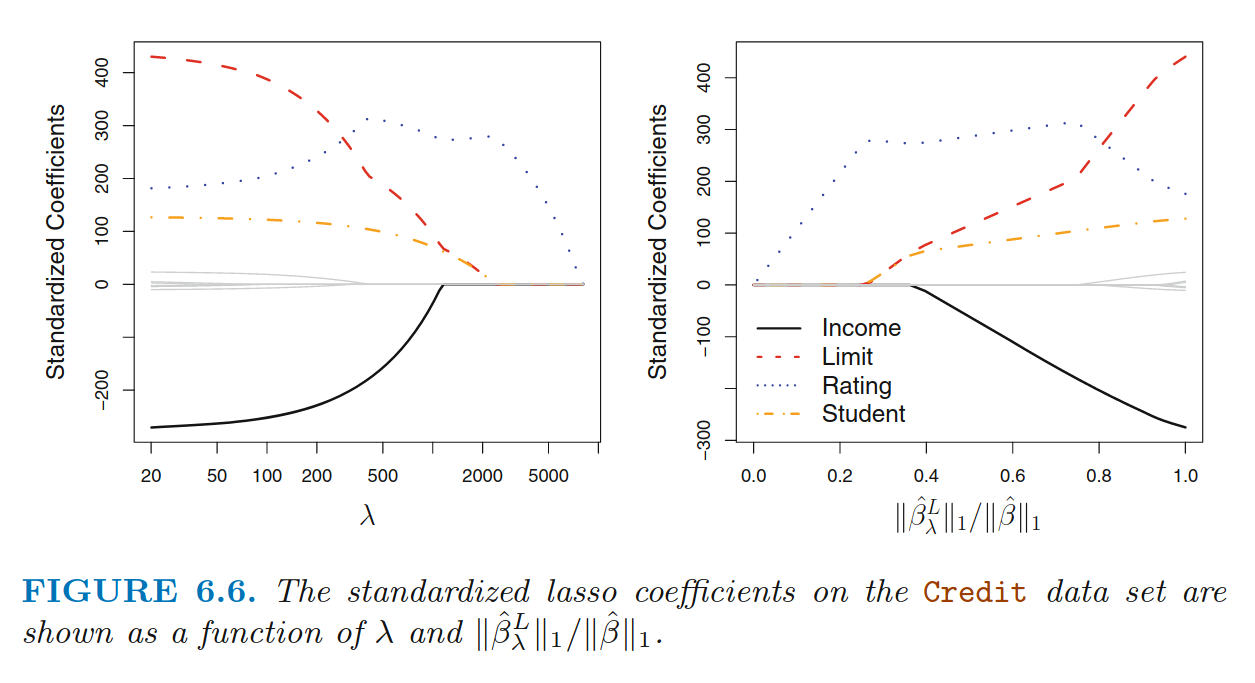
\includegraphics[width=\textwidth]{figs/standardized lasso coefficients.png}

\end{frame}

\begin{frame}{Ridge vs Lasso}
    \begin{tabular}{lll}
        & Ridge & Lasso \\ \hline
        $\lambda \to 0$ & $\hat{\beta}_{\text{Ridge}} \to \hat{\beta}_{\text{OLS}}$ & $\hat{\beta}_{\text{Lasso}} \to \hat{\beta}_{\text{OLS}}$ \\
        $\lambda \to \infty$ &  $\hat{\beta}_{\text{Ridge}} \to 0$ &  $\hat{\beta}_{\text{Lasso}} \to 0$ \\
        Norm & $l^2$-norm & $l^1$-norm \\
        Område & Hypersfär & Polytop \\
        Parametrar & Krymper och ger många små $\beta$ & Sätter många till 0 \\
        Korrelerade variabler & Krymper alla lika mycket & Sätter en till 0
    \end{tabular}
\end{frame}

\begin{frame}{Ridge vs Lasso}

    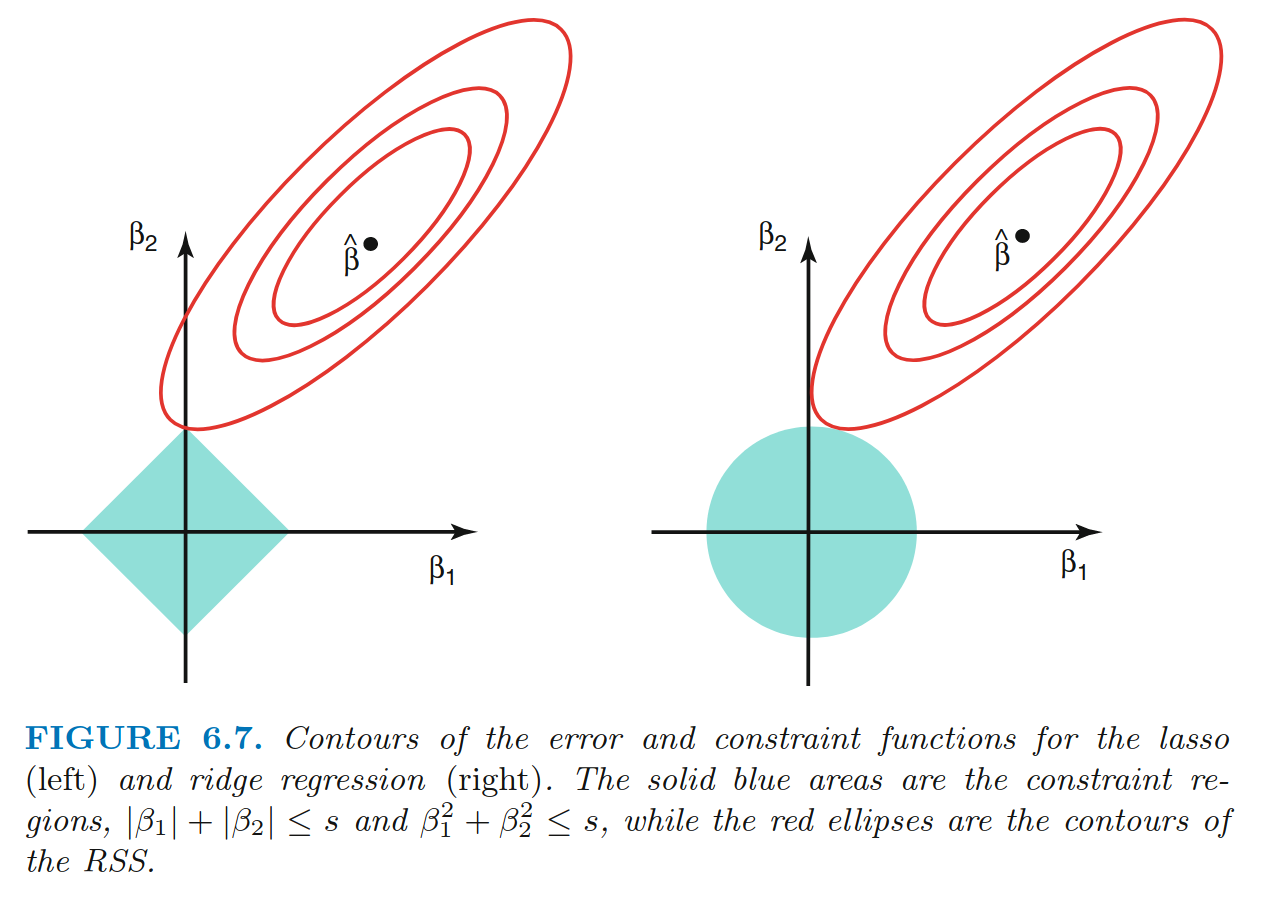
\includegraphics[width=\textwidth]{figs/Contours of the error .png}
    
\end{frame}

\begin{frame}{Ridge vs Lasso}
    
    \begin{itemize}
        \item I R, skattas enkelt med \texttt{glmnet()} eller \texttt{cv.glmnet()}.
        \item Vilken som är bäst beror på kontext.
        \item Ridge passar bra när $y$ beror på de flesta variablerna.
        \begin{itemize}
            \item Många variabler och ungefär samma effektstorlek.
        \end{itemize}
        \item Lasso passar bra när $y$ beror på bara några få variabler.
        \begin{itemize}
            \item Fåtal variabler med hög effektstorlek, resten nära 0.
        \end{itemize}
        \item Lasso kan vara lättare att tolka.
        % \item Lättare att göra inferens på parameterarna i Ridge.
        \item Vilken man ska välja får ofta avgöras empiriskt för specifika dataset.
        \item Finns många utökningar och varianter.
        \item $l^2$-norm och $l^1$-norm används som regularisering inom många olika modeller inom maskininlärning
    \end{itemize}

\end{frame}

\begin{frame}{Adaptive-Lasso}
    \begin{itemize}
        \item Låt varje parameter $\beta_j$ ha sin egen vikt $w_j$
        \begin{equation*}
            f(\beta) = \sum_{i=1}^{n}\left(y_i - \beta_0 - \sum_{j=1}^{p}\beta_j x_{ij}\right)^2 + \lambda \sum_{j=1}^{p} w_j |\beta_j|, \quad \lambda \geq 0.
        \end{equation*}
        \item Välj vikter
        \begin{equation*}
            w_j = | \hat{\beta}_{j, \text{start}} |^{-\gamma}
        \end{equation*}
        \item Ofta väljs $\gamma = 1$.
        \item Behöver startvärde $\hat{\beta}_{j,\text{start}}$, kan använda OLS eller Ridge skattning.
        \item Stora startvärden ger små vikter vilket gör att parametern krymper mindre.
        \item Finns vissa teorestiska fördelar, men kräver extra skattning.
    \end{itemize}
\end{frame}

\begin{frame}{Elasticnet regression}

    \begin{itemize}
        \item Kombinerar Ridge och Lasso.
        \item Ny hyperparameter $\alpha$ för att mixa dessa,
        \begin{equation*}
            f(\beta) = \operatorname{RSS} + \lambda \left((1-\alpha) \sum_{j=1}^{p}\beta_j^2 + \alpha \sum_{j=1}^{p}|\beta_j|  \right), \qquad \lambda \geq 0,\, 0 \leq \alpha \leq 1.
        \end{equation*}
        \item $\lambda$ är likt tidigare hur mycket regularisering vi gör.
        \item $\alpha$ väljer hur mycket vikt vid Ridge respektive Lasso.
        \item Kan tvinga vissa $\beta$ till 0, men inte lika många som Lasso.
        \item Klarar av korrelerade/grupper av variabler bättre än Lasso.
        \item Nackdel är att vi har två hyperparametrar.
    \end{itemize}
    
\end{frame}


\begin{frame}{Adaptive Elasticnet regression}

    \begin{itemize}
        \item Kombinerar Ridge, Lasso och vikter.
        \item Ny hyperparameter $\alpha$ för att mixa dessa,
        
        
        \begin{equation*}
            f(\beta) = \operatorname{RSS} + \lambda \sum_{j=1}^{p} w_j \left((1-\alpha) \frac{1}{2} \beta_j^2 + \alpha|\beta_j|  \right), \qquad \lambda \geq 0,\, 0 \leq \alpha \leq 1.
        \end{equation*}
        \item Välj vikter
        \begin{equation*}
            w_j = | \hat{\beta}_{j, \text{start}} |^{-\gamma}
        \end{equation*}
        \item Ofta väljs $\gamma = 1$.
        \item Behöver startvärde $\hat{\beta}_{j,\text{start}}$, kan använda OLS eller Ridge skattning.
        \item Två hyperparameterar: $\alpha$ och $\lambda$
    \end{itemize}
    
\end{frame}


\end{document}